\documentclass{article}%
\usepackage[T1]{fontenc}%
\usepackage[utf8]{inputenc}%
\usepackage{lmodern}%
\usepackage{textcomp}%
\usepackage{lastpage}%
\usepackage[head=40pt,margin=0.5in,bottom=0.6in]{geometry}%
\usepackage{graphicx}%
%
\title{\textbf{Venezolanos con VIH que emigran a Colombia no pueden costear sus medicinas}}%
\author{EL NACIONAL WEB}%
\date{19/10/2018}%
%
\begin{document}%
\normalsize%
\maketitle%
\textbf{URL: }%
http://www.el{-}nacional.com/noticias/salud/venezolanos{-}con{-}vih{-}que{-}emigran{-}colombia{-}pueden{-}costear{-}sus{-}medicinas\_256464\newline%
%
\textbf{Periodico: }%
EN, %
ID: %
256464, %
Seccion: %
Salud\newline%
%
\textbf{Palabras Claves: }%
Salud, Colombia, Diáspora, VIH\newline%
%
\textbf{Derecho: }%
2.1, %
Otros Derechos: %
, %
Sub Derechos: %
2.1.1\newline%
%
\textbf{EP: }%
NO\newline%
\newline%
%
\textbf{\textit{Los emigrantes con este padecimiento decieron salir de Venezuela debido a las precarias condiciones de la atención hospitalaria del país}}%
\newline%
\newline%
%
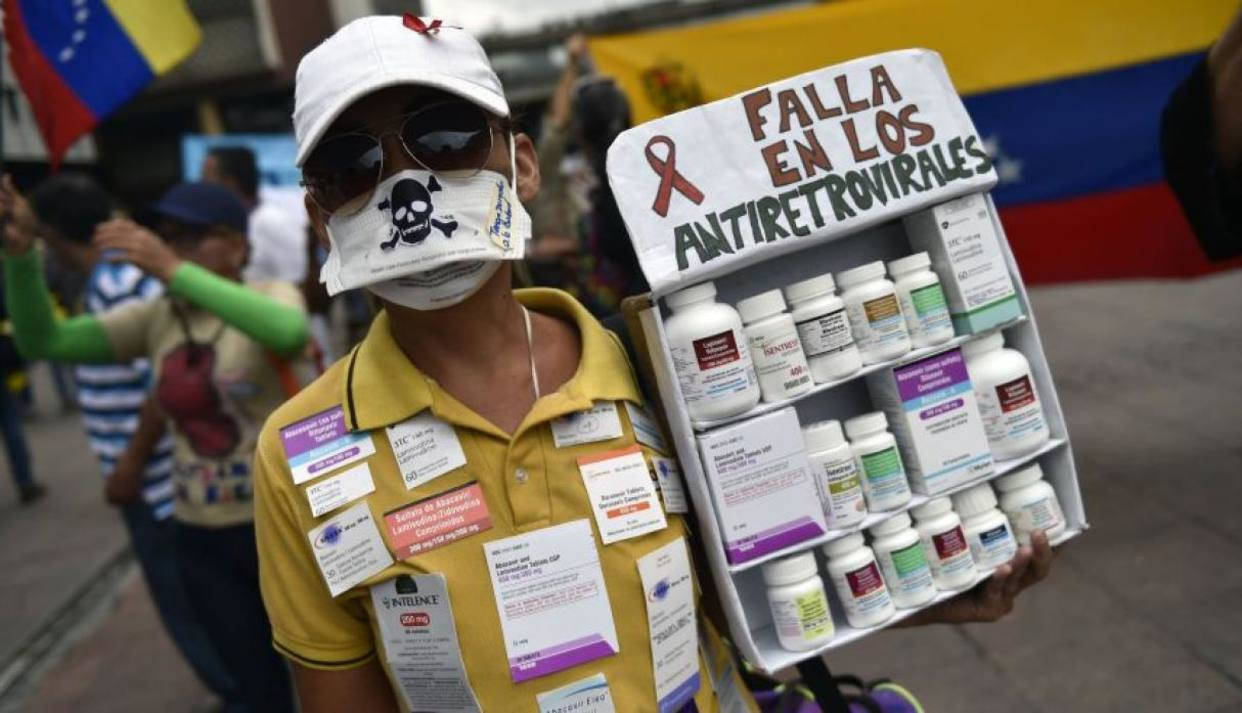
\includegraphics[width=300px]{173.jpg}%
\newline%
%
Un total de 21 venezolanos~con el Virus de la Inmunodeficiencia Humana (VIH) han emigrado a Barranquilla, Colombia de forma ilegal~con la intención de adquirir las medicinas que necesitan. Entre este grupo, hay una menor de edad.%
\newline%
%
Muchos de los inmigrantes con esta condición, dado su estatus ilegal, no tienen los recursos necesarios para comprar las medicinas que requieren para su tratamiento, indicó~NTN24.%
\newline%
%
El sector público de salud en Colombia ha intentado contabilizar estos casos entre las miles de personas que ingresan diariamente al país, pero les resulta complicado debido a que muchos de ellos temen revelar sus condición por rechazo, indicó Humberto Mejía, integrante de la Fundación Arenosa Vive.%
\newline%
%
Estos venezolanos han sido instruidos con respecto a su enfermedad para evitar contagios y problemas con respecto a su control.%
\newline%
%
La Cruz Roja de Colombia, en conjunto con las autoridades del sector salud, organizan charlas de prevención y jornadas médicas integrales para los afectados por este virus.%
\newline%
%
Lea la nota completa~aquí%
\newline%
%
\end{document}